\documentclass[11pt,a4paper]{article}

\usepackage[a4paper,margin=2.3cm]{geometry}
\usepackage[T1]{fontenc}
\usepackage{lmodern}
\usepackage{amsmath,amssymb}
\usepackage{xcolor}
\usepackage{graphicx}
\usepackage{subcaption}
\usepackage{booktabs}
\usepackage[font=small,labelfont=bf]{caption}
\usepackage[colorlinks=true,linkcolor=blue!60!black,citecolor=blue!60!black,urlcolor=blue!60!black]{hyperref}

\graphicspath{{figures/}{./}}
\numberwithin{equation}{section}
\setlength{\parskip}{3pt}

\newcommand{\bk}{\mathbf{k}}
\newcommand{\bq}{\mathbf{q}}
\newcommand{\chie}{\chi_{e}}
\newcommand{\chig}{\chi_{\rm geom}}
\newcommand{\chim}{\chi_{\rm mass}}
\newcommand{\Evhs}{E_{\rm vhs}}
\newcommand{\meV}{\,\mathrm{meV}}
\newcommand{\nm}{\,\mathrm{nm}}

\title{\textbf{Quantum Geometric Effects at the Monkey Saddle Lifshitz Point in biased Bernal Bilayer Graphene}}
\author{Rajat Shuvra Saha\\[2pt]
\small School of Physical Sciences, National Institute of Science Education and Research (NISER)\\
\small Master's thesis report}
\date{\today}

\begin{document}
\maketitle

\begin{abstract}
\noindent
At a critical inter-layer bias, $V_c\simeq 40\meV$ the three Van Hove saddles of the lowest conduction band of Bernal Bilayer Graphene merge into a single monkey saddle, a higher order Van Hove singularity with a power-law divergent density of states. We ask whether the quantum geometry of this band favors ferromagnetic fluctuations, in the sense recently proposed by Kitamura, Daido and Yanase for singular saddle point. Using the four band continuum model, we compute the Generalized Electric Susceptibility (GES), $\chie$, the $q^2$ curvature of the bare spin susceptibility, and separate it into a geometric part $\chig$ and an effective-mass part $\chim$. The monkey saddle carries a large, metric dominated quantum geometry, but near the Van Hove energy the sign of $\chie$ is controlled by the dispersion. Geometry driven ferromagnetic fluctuations, $\chie<0<\chim$, appear in well-defined windows: on the high density side $\mu-V/2\gtrsim 4.2\ meV$ at all biases studied, and at low temperature at the Van Hove energy for $V>V_C$. In these windows, $q=0$ is a local, not global, maximum of $\chi^0 (q)$
\end{abstract}

\section*{Introduction}

Van Hove Singularities are the natural place to look for electronic stabilities: a logarithmically divergent density of states enhance every susceptibility, and within a Stoner Picture, lowers the interaction strength needed for magnetism. When several ordinary saddles merge, the divergence becomes a power law and the singularity is called higher order ~\cite{Yuan2019,Shtyk2017}.\\

The usual stoner argument looks only at Band Energies. Kitamura, Daido and Yanase pointed out that the momentum dependence of the Bare Susceptibility $\chi^0(\bq)$ also carries information about the Bloch wavefunctions ~\cite{Kitamura2024}. Its curvature at $q=0$, which they call the Generalized Electric Susceptibility, splits into a term set by the Band Curvature and a term set by the quantum geometry of the bands. For a singular saddle with a band touching, the geometric term alone can turn $q=0$ into a maximum of $\chi^0(\bq)$, so the uniform (Ferromagnetic) channel dominates. The quantum metric thereby enters the physics of magnetism in the same way it is known to enter flat-band superconductivity  ~\cite{Torma2022}.\\

The Monkey Saddle is a natural test of this idea. It has no band touching, but it sits at the point where two inter-band channels balance, and we shall see that the critical band carries a large quantum metric there. We are addressing three things here:

\begin{itemize}
    \item What is the quantum geometry of the critical band, and how does it change with bias?
    \item How large is $\chig$ compared with $\chim$ near the Monkey Saddle?
    \item Are there regions of chemical potential and temperature where ferromagnetic fluctuations exist only because of geometry?

\end{itemize}

Section~\ref{sec:model} introduces the model and the three saddle phases, Sec.~\ref{sec:geometry} the quantum geometry, and Sec.~\ref{sec:ges} the GES. Our results follow in Sec.~\ref{sec:results}.
    
\section{Model and the monkey saddle}\label{sec:model}

We use the four-band continuum Hamiltonian of Bernal Bilayer Graphene near valley $K$~\cite{McCann2013}, in the basis $(A_1,B_1,A_2,B_2)$, 
\begin{equation}
H(\bk)=\begin{pmatrix}
V/2 & v\pi^\dagger & 0 & v_3\pi\\
v\pi & V/2 & \gamma_1 & 0\\
0 & \gamma_1 & -V/2 & v\pi^\dagger\\
v_3\pi^\dagger & 0 & v\pi & -V/2
\end{pmatrix},\qquad \pi=k_x+ik_y,
\label{eq:H}
\end{equation}
with $v=0.658\,$eV\,nm, $\gamma_1=0.40\,$eV, $v_3=0.1\,v$ and interlayer bias $V$. We study the lowest conduction band, band~3 counted from below, which at $\bk=0$ is the pure $A_1$ orbital
at energy $V/2$. Because $H$ is linear in $\bk$, the velocity matrices $\partial_{k_i}H$ are constant. This makes every derivative below used an exact finite sum over states, which is very convenient both analytically and numerically.\\

Eliminating the dimer orbitals $(B_1,A_2)$ gives, to leading order (Appendix~\ref{app:dispersion}),
\begin{equation}
\varepsilon_3(\bk)-\frac V2\simeq \alpha(V)\,k^2-A\,k^3\cos3\varphi+B\,k^4,\qquad
\alpha(V)=\frac{v_3^2}{V}-\frac{v^2V}{\gamma_1^2}.
\label{eq:disp}
\end{equation}
The $k^2$ coefficient is a competition between direct trigonal-warping hopping to $B_2$, which pushes the band up, and virtual hopping through the dimer, which pushes it down. It vanishes at
\begin{equation}
V_c=\frac{\gamma_1v_3}{v}=40\meV .
\end{equation}
At $V=V_c$ the cubic term $A=2v^3/\gamma_1^2$ fixes the shape and the quartic term $B=v^5/(\gamma_1^3v_3)$ takes over at the crossover scales
\begin{equation}
k_*=A/B=0.122\nm^{-1},\qquad E_*=A^4/B^3=6.40\meV .
\end{equation}
Throughout we use $\delta\equiv V/V_c$.

\begin{figure}[t]
\centering
\begin{minipage}[c]{0.36\textwidth}
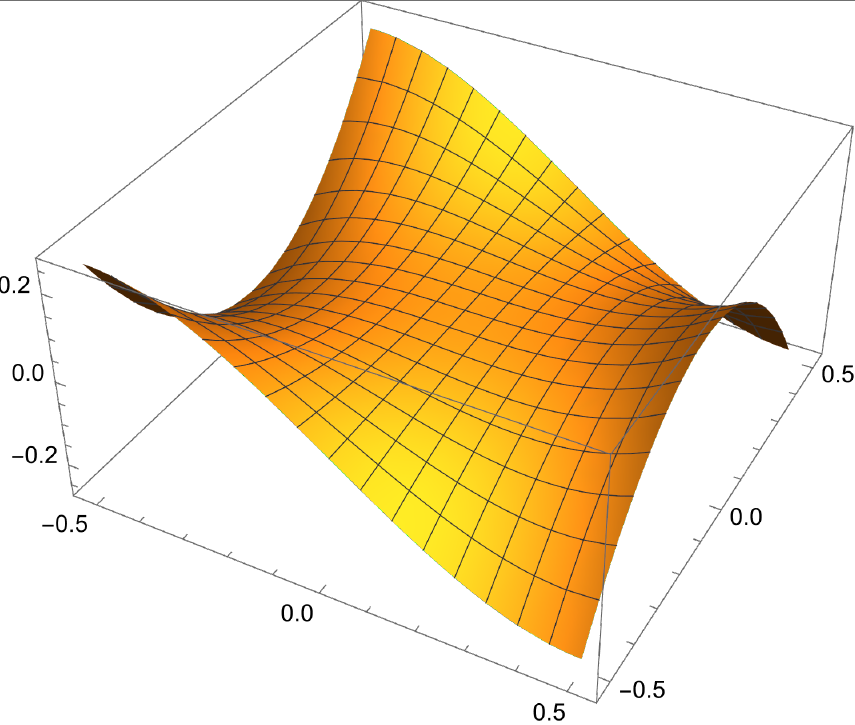
\includegraphics[width=\linewidth]{Monkey_Saddle_3D_Plot.png}
\end{minipage}\hfill
\begin{minipage}[c]{0.6\textwidth}
\caption{The monkey saddle. Dispersion $\varepsilon_3(\bk)-V_c/2$ of the critical band at $V=V_c$ near $\bk=0$. The surface rises along three directions and falls along the three in between, the cubic shape $-Ak^3\cos3\varphi$ of Eq.~\eqref{eq:disp}. The Hessian vanishes at the centre, so the density of states diverges as $|E-E_c|^{-1/3}$ rather than logarithmically.}
\label{fig:monkey}
\end{minipage}
\end{figure}

For $\delta\neq1$ and small $|\alpha|$, Eq.~\eqref{eq:disp} has three ordinary saddles at $|\bk_s|=2|\alpha|/3A$ with energy
\begin{equation}
\Evhs-\frac V2\simeq\frac{4\alpha^3}{27A^2}.
\label{eq:Evhs}
\end{equation}
The three saddle phases are shown in Fig.~\ref{fig:phases}. Critical points are located exactly along the mirror lines and classified by the Hessian of $\varepsilon_3$ (Appendix~\ref{app:numerics}); Table~\ref{tab:crit} lists them.
\begin{itemize}
\item For $\delta<1$, $\bk=0$ is a local minimum surrounded by three saddles on $\varphi=0,\pm2\pi/3$.
\item At $\delta=1$ the saddles have merged into the monkey saddle.
\item For $\delta>1$, $\bk=0$ becomes a local maximum and the saddles reappear rotated by $\pi/3$.
\end{itemize}
In all three phases the band bottom lies in three minivalleys at $|\bk|\approx0.6$--$0.9\,k_*$. At $\delta=1$ the density of states diverges as $\nu(E)\simeq0.0615\,A^{-2/3}|E-E_c|^{-1/3}$ (Appendix~\ref{app:dispersion}), the property that makes the monkey saddle attractive for instabilities.

\begin{figure}[t]
\centering
\begin{subfigure}{\textwidth}\centering
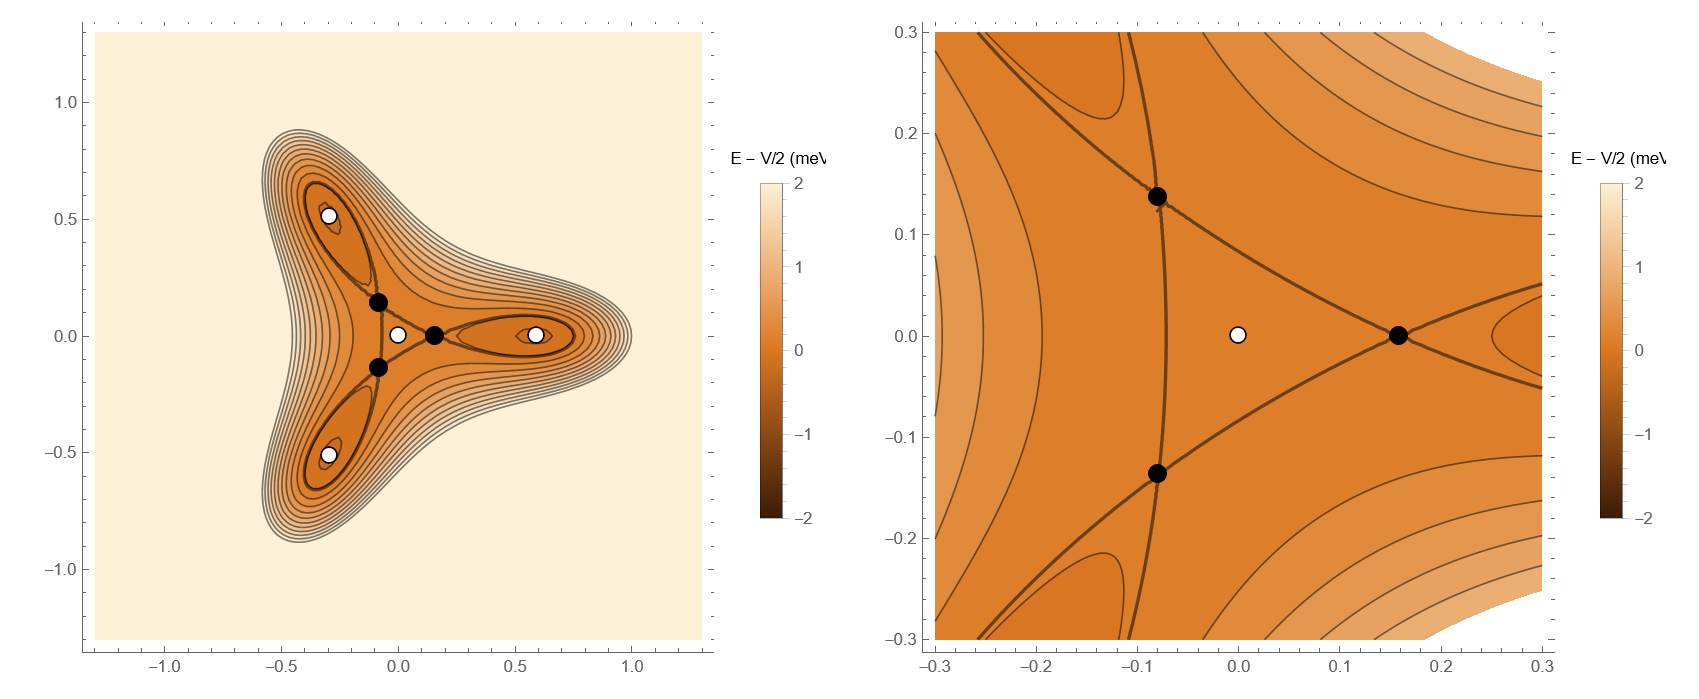
\includegraphics[width=0.82\textwidth]{Undergapped_state.png}
\caption{$\delta=0.5$: minimum at $\bk=0$ (white) and three saddles (black).}
\end{subfigure}\\[4pt]
\begin{subfigure}{0.49\textwidth}\centering
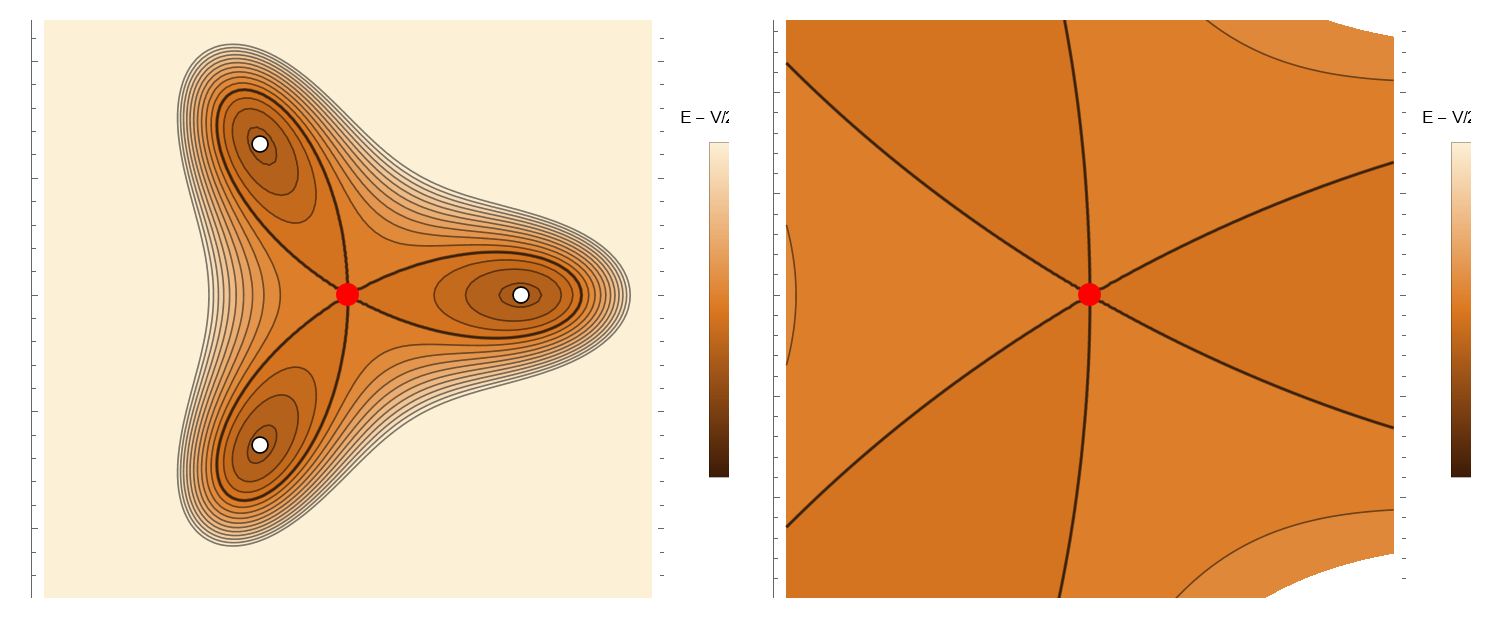
\includegraphics[width=\textwidth]{Delta=1.0.png}
\caption{$\delta=1.0$: monkey saddle (red).}
\end{subfigure}\hfill
\begin{subfigure}{0.49\textwidth}\centering
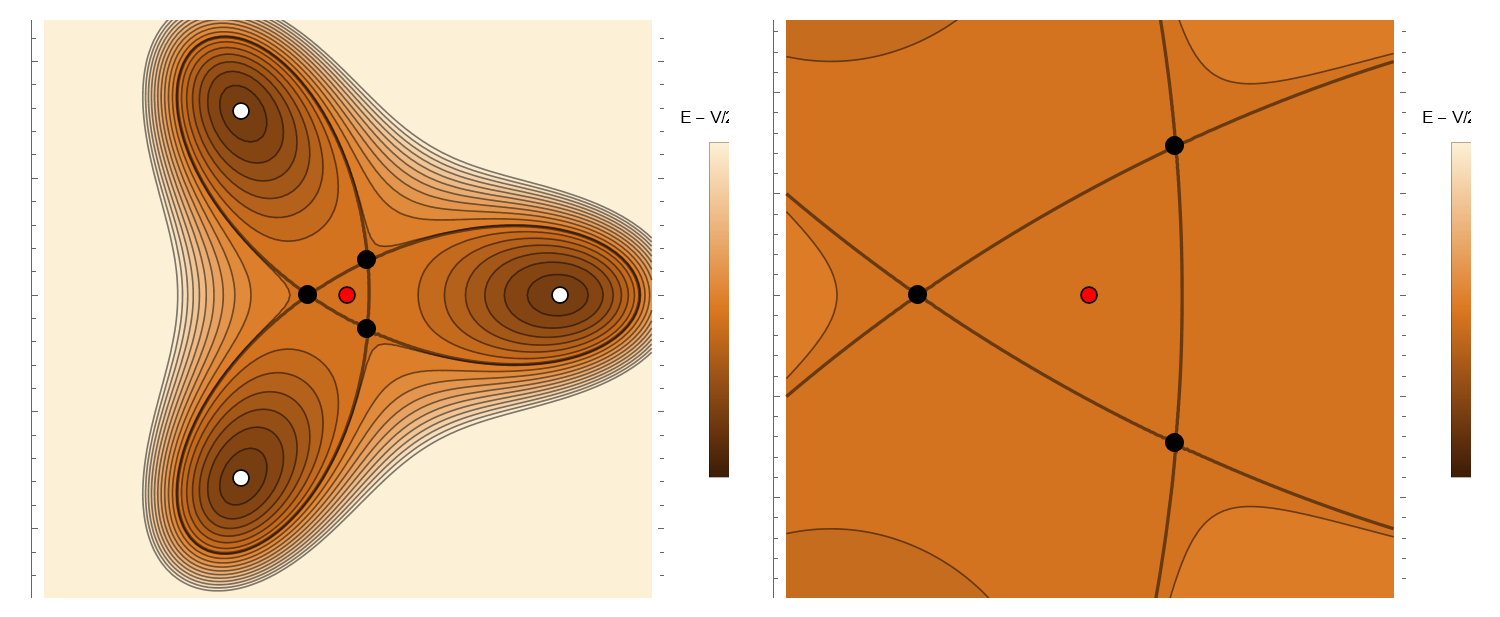
\includegraphics[width=\textwidth]{Overgapped.png}
\caption{$\delta=1.5$: maximum at $\bk=0$ (red), saddles rotated by $\pi/3$.}
\end{subfigure}
\caption{The three saddle phases of the critical band. Colour: $\varepsilon_3-V/2$ in meV, clipped at $\pm2\meV$. Axes: $k_{x,y}/k_*$. In each pair the right panel is a zoom $|k|\le0.3\,k_*$. The thick contour is the van Hove energy, and white circles mark the minivalley minima.}
\label{fig:phases}
\end{figure}

\begin{table}[t]
\centering\small
\begin{tabular}{@{}cccccc@{}}
\toprule
$\delta$ & position & $|\bk|/k_*$ & $E-V/2$ (meV) & Hessian eigenvalues (eV\,nm$^2$) & type \\
\midrule
0.5 & $\bk=0$ & 0 & 0 & $0.325,\ 0.325$ & minimum\\
0.5 & $\varphi=0$ & 0.158 & $+0.0174$ & $-0.237,\ 1.230$ & saddle ($\times3$)\\
0.5 & $\varphi=0$ & 0.590 & $-0.239$ & $0.875,\ 4.580$ & minivalley ($\times3$)\\
1.0 & $\bk=0$ & 0 & 0 & $0,\ 0$ & monkey saddle\\
1.0 & $\varphi=0$ & 0.745 & $-0.657$ & $0.943,\ 2.871$ & minivalley ($\times3$)\\
1.5 & $\bk=0$ & 0 & 0 & $-0.180,\ -0.180$ & maximum\\
1.5 & $\varphi=\pi$ & 0.170 & $-0.0140$ & $-0.440,\ 0.213$ & saddle ($\times3$)\\
1.5 & $\varphi=0$ & 0.909 & $-1.336$ & $1.097,\ 2.314$ & minivalley ($\times3$)\\
\bottomrule
\end{tabular}
\caption{Critical points of $\varepsilon_3$ from exact diagonalisation. In every phase the Morse count, minima $-$ saddles $+$ maxima, equals one.}
\label{tab:crit}
\end{table}

\section{Quantum Geometry of the Critical Band}\label{sec:geometry}
The quantum geometric tensor of band $n$, $Q^n_{\mu\nu}=\langle\partial_\mu u_n|(1-|u_n\rangle\langle u_n|)|\partial_\nu u_n\rangle=g^n_{\mu\nu}-\tfrac i2\Omega^n_{\mu\nu}$, contains the quantum metric $g$ and the Berry curvature $\Omega$~\cite{Provost1980}. For a Hamiltonian linear in $\bk$ both follow from the interband velocity matrix elements $v^\mu_{nm}=\langle n|\partial_\mu H|m\rangle$:
\begin{equation}
g^n_{\mu\nu}=\sum_{m\neq n}\frac{\mathrm{Re}\,v^\mu_{nm}v^\nu_{mn}}{(\varepsilon_n-\varepsilon_m)^2},\qquad
\Omega^n_{xy}=-2\sum_{m\neq n}\frac{\mathrm{Im}\,v^x_{nm}v^y_{mn}}{(\varepsilon_n-\varepsilon_m)^2}.
\label{eq:qgt}
\end{equation}
At $\bk=0$ only two channels contribute, the same two that compete in $\alpha(V)$. Appendix~\ref{app:geometry} shows that
\begin{equation}
g_{xx}=g_{yy}=\underbrace{\frac{v_3^2}{V^2}}_{B_2}+\underbrace{\frac{v^2(\gamma_1^2+V^2)}{\gamma_1^4}}_{\rm dimer},\qquad
\Omega_{xy}=\frac{2v_3^2}{V^2}-\frac{2v^2(\gamma_1^2+V^2)}{\gamma_1^4},\qquad g_{xy}=0 .
\label{eq:gOmega}
\end{equation}
The relative sign is the main point. The $B_2$ channel couples through $\pi$ and the dimer channel through $\pi^\dagger$, so they carry opposite chirality. Each saturates the bound $|\Omega|\le2\sqrt{\det g}$ on its own; their metrics add while their curvatures cancel.

Near $V_c$ the two channels are almost equal in size, which is the same balance that makes $\alpha(V_c)=0$ up to a correction of order $V^2/\gamma_1^2$. The critical band therefore carries a large quantum metric with almost no Berry curvature (Table~\ref{tab:geo}): $g=5.44\nm^2$ at $V_c$, half of it from the remote dimer bands, while $\Omega$ passes through zero at $V=0.995\,V_c$. Away from $\bk=0$ the metric and curvature are concentrated in three lobes near $|\bk|\approx k_*$, beyond the tips of the van Hove contour. The geometry relevant to the monkey saddle is thus \emph{metric dominated}. This is precisely the ingredient that enters the GES.

\begin{table}[t]
\centering\small
\begin{tabular}{@{}ccccc@{}}
\toprule
$\delta$ & $\alpha$ (eV\,nm$^2$) & $g_{xx}(\bk=0)$ (nm$^2$) & $\Omega_{xy}(\bk=0)$ (nm$^2$) & dimer share of $g$\\
\midrule
0.5 & $+0.162$ & 13.54 & $+16.22$ & 0.20\\
1.0 & $0$ & 5.44 & $-0.05$ & 0.50\\
1.5 & $-0.090$ & 3.97 & $-3.13$ & 0.69\\
\bottomrule
\end{tabular}
\caption{Effective-mass coefficient and quantum geometry of band 3 at $\bk=0$, Eqs.~\eqref{eq:disp} and \eqref{eq:gOmega}. Exact diagonalisation agrees to all digits shown.}
\label{tab:geo}
\end{table}





\section{Generalized electric Susceptibility}\label{sec:ges}
The bare spin susceptibility (per spin and valley) is
\begin{equation}
\chi^0(\bq)=-\sum_{nm}\int\!\frac{d^2k}{(2\pi)^2}\,
\frac{f(\varepsilon_{n,\bk_-})-f(\varepsilon_{m,\bk_+})}{\varepsilon_{n,\bk_-}-\varepsilon_{m,\bk_+}}\,
\big|\langle u_{n,\bk_-}|u_{m,\bk_+}\rangle\big|^2,\qquad \bk_\pm=\bk\pm\bq/2 .
\label{eq:bubble}
\end{equation}
Following Ref.~\cite{Kitamura2024} the GES is its curvature at the origin,
\begin{equation}
\chie\equiv\lim_{\bq\to0}\partial_{q_x}^2\chi^0(\bq),\qquad
\chi^0(\bq)\simeq\chi^0(0)\big(1-\ell^2q^2\big),\qquad \ell^2=-\frac{\chie}{2\chi^0(0)} .
\label{eq:GESdef}
\end{equation}
$C_3$ symmetry makes the curvature tensor isotropic. A negative $\chie$ means that $q=0$ is a maximum of $\chi^0$; within RPA, $\chi_s=\chi^0_S/(1-U\chi^0_s)$, the Stoner instability then occurs first in the uniform channel, and the paramagnet has ferromagnetic fluctuations.
Expanding Eq.~\eqref{eq:bubble} to order $q^2$ (Appendix~\ref{app:ges}) gives $\chie=\chig+\chim$, with
\begin{align}
\chig&=2\sum_n\int\!\frac{d^2k}{(2\pi)^2}\Big[\frac{f'(\varepsilon_n)}{2}\,g^{n}_{K}+f(\varepsilon_n)\,X_n\Big], \label{eq:chig}\\
\chim&=-2\sum_n\int\!\frac{d^2k}{(2\pi)^2}\,\frac{f''(\varepsilon_n)}{12}\,\big[m_n^{-1}\big], \label{eq:chim}
\end{align}
which is the form given by Kitamura \emph{et al.} Here $g_K$ is twice the direction-averaged standard metric of Eq.~\eqref{eq:qgt}, $X_n$ is the interband (positional-shift) term and $[m_n^{-1}]$ is the inverse effective mass (explicit forms in Appendix~\ref{app:ges}). Two observations organise everything that follows.

\begin{enumerate}
\item The Fermi-surface metric term is always negative, because $f'\le0$. Geometry therefore always pushes towards ferromagnetism at the Fermi surface; the Fermi-sea term $X_n$ can partially compensate.
\item $f''(\varepsilon-\mu)$ is odd about $\mu$, so $\chim$ measures the \emph{imbalance} of band curvature just below and just above $\mu$. Near a saddle both sides are large and of opposite curvature, so $\chim$ is large and changes sign as $\mu$ crosses $\Evhs$.
\end{enumerate}

We call a ferromagnetic fluctuation \emph{geometry driven} when $\chie<0$ but $\chim>0$, i.e.\ when the dispersion alone would make $q=0$ and a minimum of $\chi^0$. \\\\

For the sake of our simulations, we would like to declare that all integrals are evaluated on Gauss Legendre Polar Grids with full Fermi functions for all four bands; The numerical details and convergence of grids are in Appendix ~\cite{app:numerics}. Results are given per spin and per valley and  the $K'$ valley contributes identically by time reversal symmetry.

\section{Results}\label{sec:results}

Figure ~\ref{fig:gesmu} shows the three components against chemical potential at $T=0.1\meV$ for $\delta=0.8$, $1$ and $1.2$.
\emph{Near the van Hove energy} (top row) both components are tens of $\text{eV}^{-1}$. $\chim$ changes sign at $\Evhs$, as we expected, and controls the sign of $\chie$. Just below $\Evhs$, there is a ferromagnetic window, but it is mostly dispersion driven (grey). Quantum Geometry only widens it, adding the narrow orange strip at its upper edge.


\emph{On the high-density side} (bottom row) the picture changes. The components are an order of magnitude smaller and $\chim$ stays positive, but $\chig$ is negative and larger. From $\mu-V/2\approx4.2\meV$ upward $\chie<0$ purely because of geometry. This window is essentially independent of bias.

At $\mu-V/2=8\meV$ and $V=V_c$ we find $\chie=-0.30$ and $\chim=+1.57\,$eV$^{-1}$, so geometry turns a dip of the bubble at $q=0$ ($\ell^2=-6.8\nm^2$) into a peak ($\ell^2=+1.3\nm^2$).

\begin{figure}[h!]
\centering
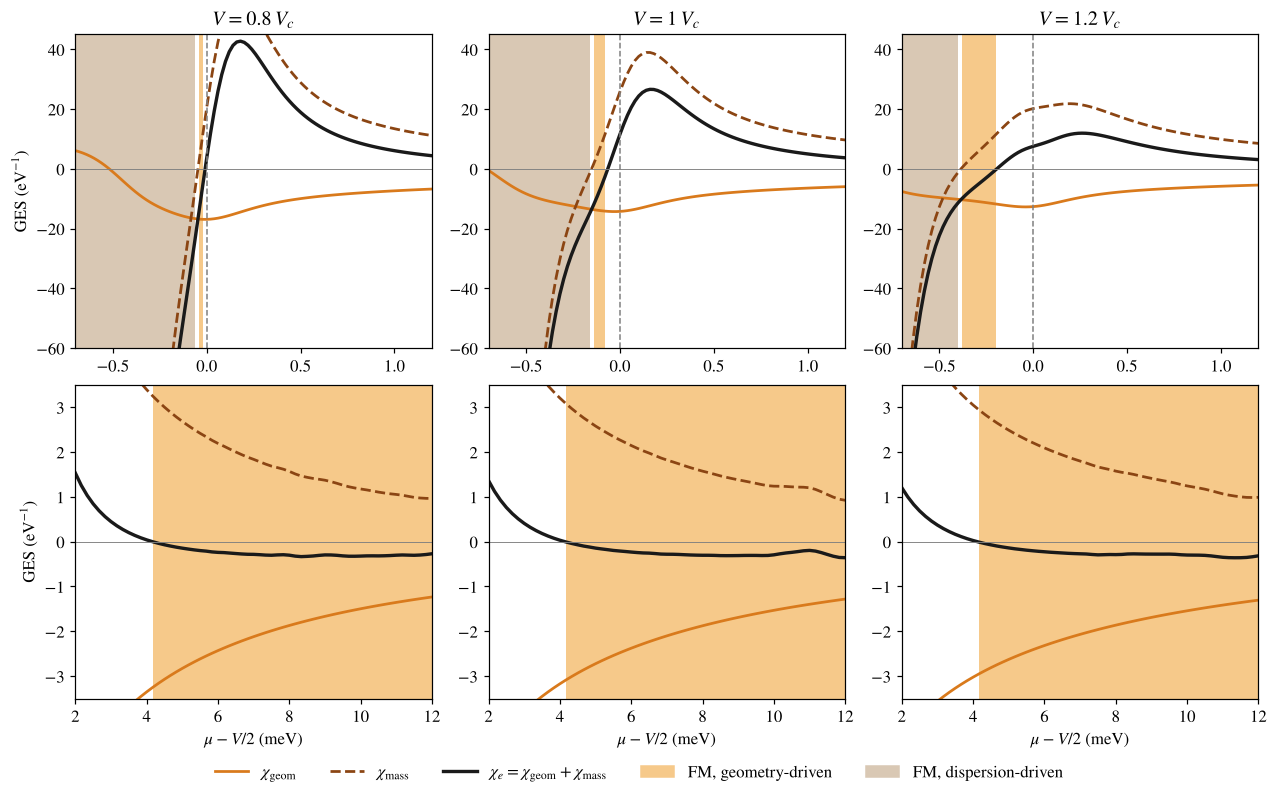
\includegraphics[width=\textwidth]{GES_ipynb_Biased.png}
\caption{GES components against chemical potential at $T=0.1\meV$. Top: near the van Hove energy (dashed vertical line). Bottom: high-density side. Orange shading: geometry-driven ferromagnetic fluctuation ($\chie<0<\chim$). Grey: dispersion-driven ($\chie<0$, $\chim<0$).}
\label{fig:gesmu}
\end{figure}

\subsection{Temperature dependence at the van Hove energy}

Figure~\ref{fig:Tsweep} follows the three components at $\mu=\Evhs$ from $1.16$ to $116\,$K ($0.1$--$10\meV$) for the three saddle phases. Over this range the thermal window reaches the valence band, which is only $V$ away, so all four bands are treated with full Fermi functions.

The behaviour is qualitatively different in the three phases.
\begin{itemize}
\item \textbf{$\delta=0.5$.} $\chim$ is large and negative at all temperatures, with a minimum of $-65\,$eV$^{-1}$ near $2\,$K. $\chie$ reaches $-83\,$eV$^{-1}$. The ferromagnetic tendency is strong but entirely dispersion driven.
\item \textbf{$\delta=1$.} At the lowest temperature $\chim=+26\,$eV$^{-1}$ outweighs $\chig=-14\,$eV$^{-1}$, so $\chie>0$. $\chim$ changes sign near $2.5\,$K, and $\chie$ is negative between $1.8$ and $79\,$K. Geometry decides the sign only in the narrow interval $1.9$--$2.5\,$K.
\item \textbf{$\delta=1.5$.} $\chie$ is negative over the whole range. Below $5\,$K, $\chim>0$ while $\chie<0$: at the van Hove energy above $V_c$, the low-temperature ferromagnetic tendency is \emph{geometry driven}.
\end{itemize}
In all three cases $\chig$ is most negative at low temperature and turns positive at high temperature (at $16$, $34$ and $63\,$K respectively). The cause is thermal occupation of the valence band, which makes the positive Fermi-sea term dominate.

\begin{figure}[t]
\centering
\begin{subfigure}{0.329\textwidth}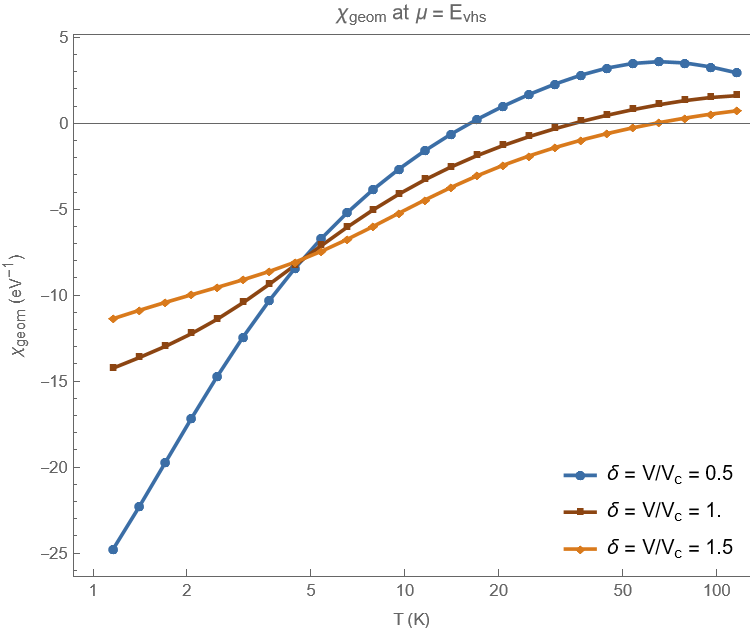
\includegraphics[width=\textwidth]{chi_geom_Temperature_Scan_Biased.png}\caption{$\chig$}\end{subfigure}\hfill
\begin{subfigure}{0.329\textwidth}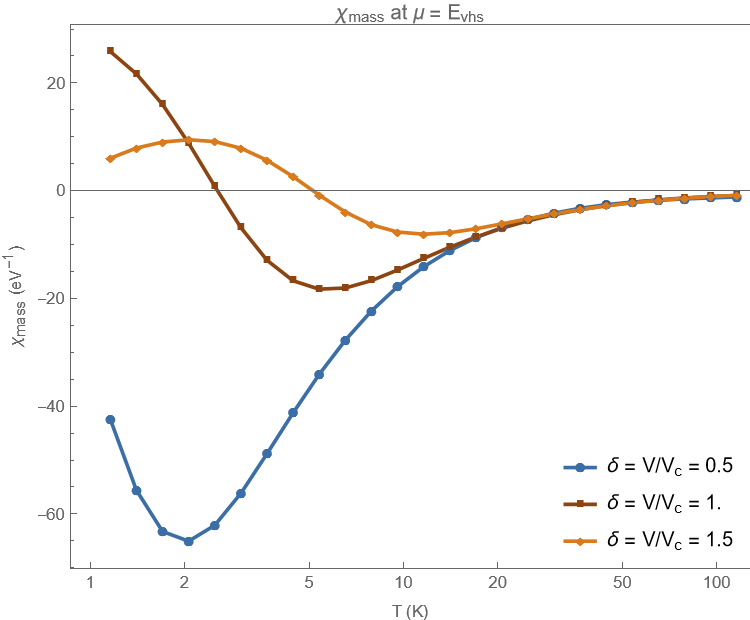
\includegraphics[width=\textwidth]{chi_mass_Temperature_Scan_Biased.png}\caption{$\chim$}\end{subfigure}\hfill
\begin{subfigure}{0.329\textwidth}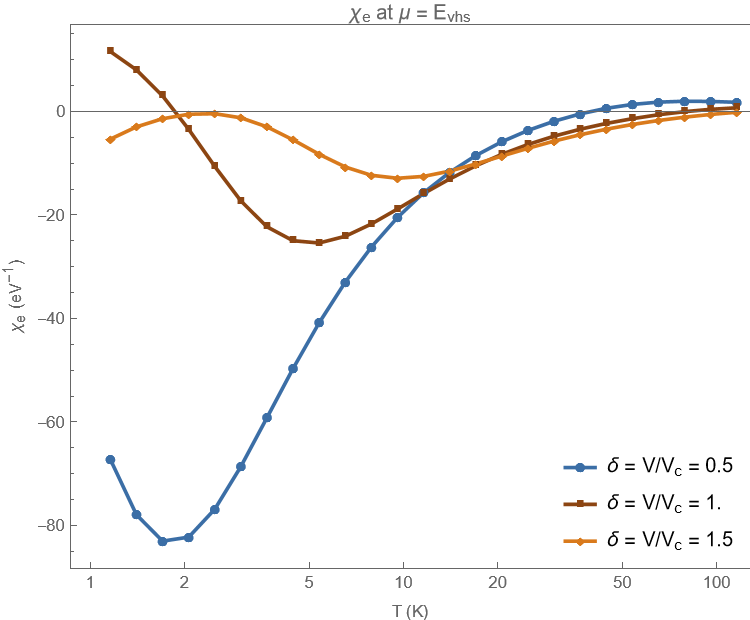
\includegraphics[width=\textwidth]{chi_total_temp_scan_biased.png}\caption{$\chie=\chig+\chim$}\end{subfigure}
\caption{Temperature dependence of the GES at $\mu=\Evhs$ for $\delta=0.5$, $1$ and $1.5$, from $1.16$ to $116\,$K.}
\label{fig:Tsweep}
\end{figure}

Figure~\ref{fig:chi0} puts these numbers in context. At $\mu=\Evhs$ and $V=V_c$ the uniform susceptibility follows $\chi^0(0)\propto T^{-1/3}$ below about $0.1\meV$ (local exponent $-0.34$). The prefactor agrees with the analytic result $\chi^0(0)\simeq0.0702\,A^{-2/3}T^{-1/3}$ of Appendix~\ref{app:dispersion} to better than $1\%$. It steepens at higher $T$, once the thermal window reaches the minivalley band bottom. In the high-density window the sign difference between the full and dispersion-only GES is robust: $\chie\approx-0.3$ against $\chim\approx+1.6\,$eV$^{-1}$ for every temperature and bias shown.

\begin{figure}[t]
\centering
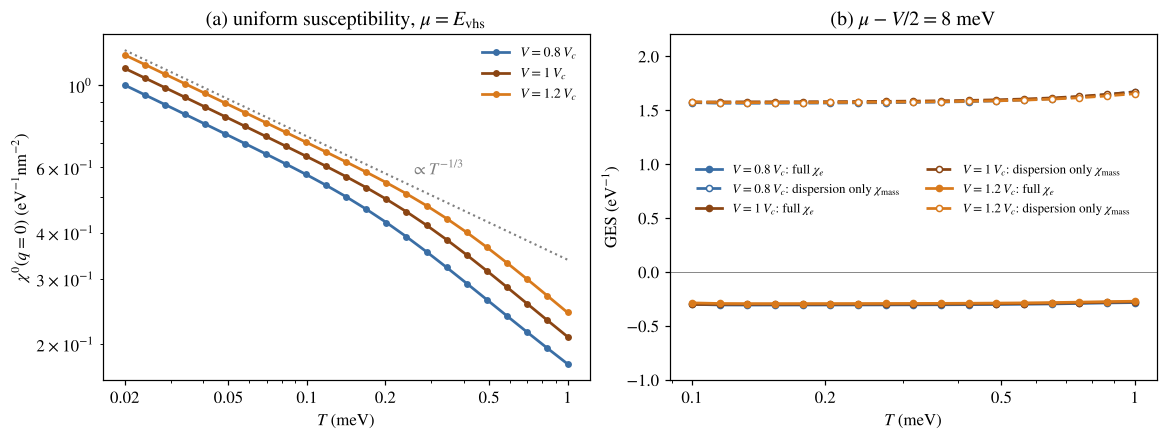
\includegraphics[width=\textwidth]{uniform_susceptibility_ipynb.png}
\caption{(a) Uniform susceptibility at the van Hove energy; dotted line $\propto T^{-1/3}$. (b) GES at $\mu-V/2=8\meV$. Solid: full $\chie$. Dashed: dispersion only, $\chim$. The three biases nearly coincide.}
\label{fig:chi0}
\end{figure}

\subsection{Direct test at finite $q$}
The GES is a statement about the curvature of $\chi^0(q)$ at the origin. To test both the decomposition of channels and the physical meaning, we evaluate ~\eqref{eq:bubble} directly at finite $q\hat{\mathbf{x}}$ for $V=V_c$, $\mu-V/2=8\meV$ and $T=0.2 \meV$.\\  

We compare the full four-band model with a geometrically trivial model, which has the same band energies but overlaps replaced by $\delta_{nm}$ (Fig.~\ref{fig:finiteq}).\\


The small-$q$ curvatures are $-0.152$ (full) and $+0.790$ (trivial). The GES formulas give $\chie/2=-0.151$ and $\chim/2=+0.788$, which confirms Eqs.~\eqref{eq:chig}--\eqref{eq:chim} independently. With geometry $q=0$ is a maximum; without it, a minimum.\\

The maximum at $q=0$ is only local. The bubble has its global maximum at $q\approx0.28\nm^{-1}$, about $15\%$ above $\chi^0(0)$. Within RPA an instability at this filling would therefore first appear at finite wavevector.

\begin{figure}[t]
\centering
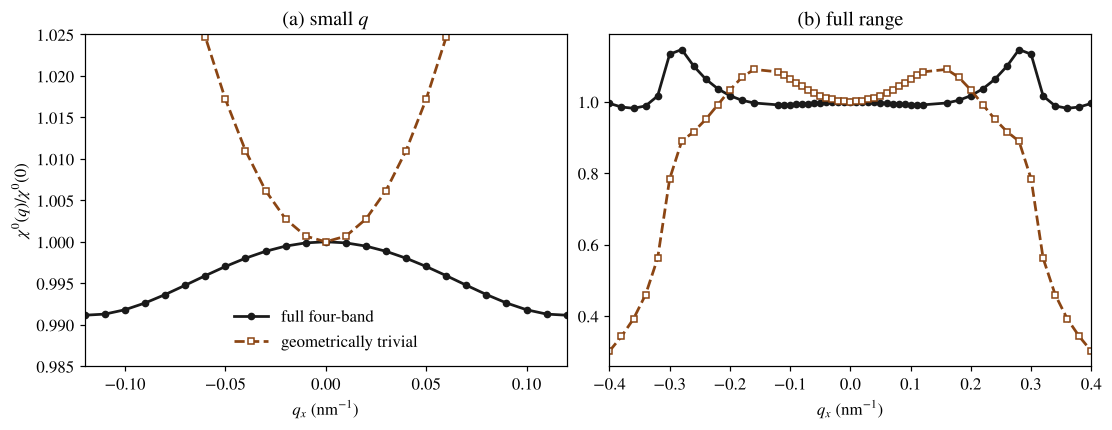
\includegraphics[width=0.92\textwidth]{fullfour_band_comparison_ipynb.png}
\caption{Bare susceptibility at finite $q$ for $V=V_c$, $\mu-V/2=8\meV$ and $T=0.2\meV$. Full four-band model (solid) and geometrically trivial model (dashed). (a) Small $q$: geometry turns the minimum at $q=0$ into a maximum. (b) Full range: the global maximum lies at $q\approx0.28\nm^{-1}$.}
\label{fig:finiteq}
\end{figure}

\subsection{Phase Diagrams of Quantum Geometry driven fluctuations}

Figure~\ref{fig:map} summarises the classification at $V=V_c$ in the $(\mu,T)$ plane. Near the monkey saddle the dispersion-driven region dominates, and the geometry-driven region is a thin band along its boundary that moves to higher $\mu$ as $T$ grows. On the high-density side the geometry-driven region is large and sharply bounded at $\mu-V/2\approx4.2\meV$, a boundary that moves only slightly up to $T\approx0.7\meV$.

\begin{figure}[t]
\centering
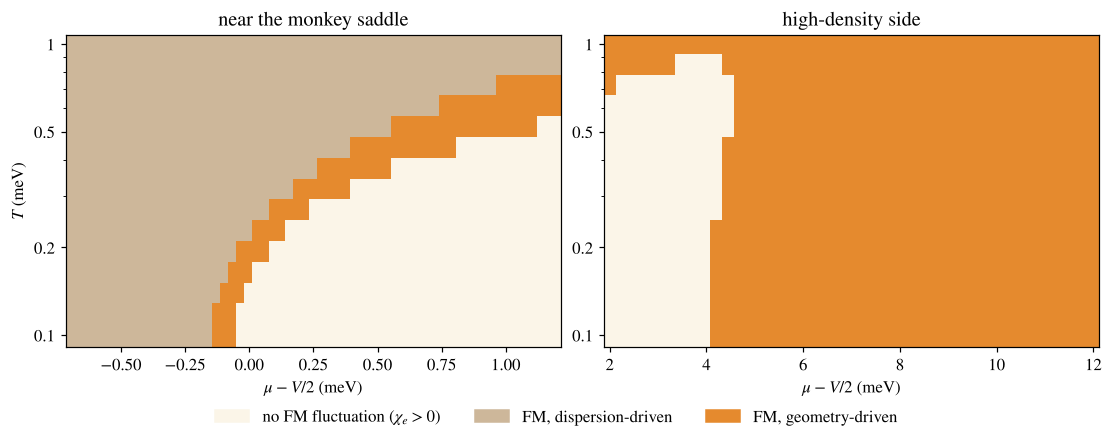
\includegraphics[width=0.92\textwidth]{Monkey_Saddle_Phase_Diagram.png}
\caption{Character of the $q=0$ response at $V=V_c$. Orange: geometry-driven ferromagnetic fluctuation ($\chie<0<\chim$). Brown: dispersion-driven ($\chie<0$, $\chim<0$). Cream: $q=0$ is a minimum of $\chi^0$.}
\label{fig:map}
\end{figure}

\section{Discussion and conclusions}\label{sec:conclusions}

We have studied the critical conduction band of biased bilayer graphene near its monkey saddle (Figs.~\ref{fig:monkey} and~\ref{fig:phases}). As the bias crosses $V_c$, three ordinary saddles merge at $\bk=0$ and reappear rotated by $\pi/3$, and at $V_c$ the density of states diverges as $|E-E_c|^{-1/3}$. The quantum geometry of this band is unusual. The two interband channels whose competition sets the effective mass have opposite chirality, so they add in the quantum metric but cancel in the Berry curvature. The monkey saddle therefore carries a large, almost purely metric geometry, with $g\simeq5.4\nm^2$ at $\bk=0$ and $\Omega_{xy}\approx0$ (Table~\ref{tab:geo}). This is precisely the ingredient that enters the generalized electric susceptibility.

Its effect on the spin response is selective. Near the van Hove energy the effective-mass term is large and changes sign, and it controls $\chie$; geometry only moves the edges of the ferromagnetic window (Fig.~\ref{fig:gesmu}, top). On the high-density side, $\mu-V/2\gtrsim4.2\meV$, the mass term stays positive but is outweighed by $\chig$, so the ferromagnetic tendency there is driven by geometry alone, at all biases studied (Fig.~\ref{fig:gesmu}, bottom, and Fig.~\ref{fig:chi0}b). The temperature sweeps at $\mu=\Evhs$ (Fig.~\ref{fig:Tsweep}) distinguish the three saddle phases. Below $V_c$ the fluctuations are strong but purely dispersive. At $V_c$ geometry decides the sign only near $2\,$K. Above $V_c$ it alone produces $\chie<0$ for $T\lesssim5\,$K. At higher temperatures, thermal occupation of the valence band turns $\chig$ positive. The uniform susceptibility follows the analytic $T^{-1/3}$ law to within $1\%$ (Fig.~\ref{fig:chi0}a), and a direct finite-$q$ calculation reproduces both $\chie$ and $\chim$ (Fig.~\ref{fig:finiteq}). That calculation also shows that the geometric peak at $q=0$ is only local: a larger maximum near $q\approx0.28\nm^{-1}$ means an RPA instability at this filling would first develop at finite wavevector. The resulting picture at $V_c$ is summarised in Fig.~\ref{fig:map}.

In contrast to the singular saddle point of Kitamura \emph{et al.}, where the metric diverges at a band touching and dominates the response (Fig.~\ref{fig:bench}), the monkey saddle is gapped and its metric remains finite. Quantum geometry is sizeable here but acts as a correction to a dispersion-dominated response, and it decides the sign of $\chie$ only where the dispersion is nearly neutral: at high density, and just above $V_c$ at low temperature. Natural extensions are to include both valleys and vertex corrections beyond RPA, to follow the finite-$q$ maximum into an ordered state, and to compare with the isospin-polarised phases observed experimentally~\cite{Zhou2022}.



\begin{thebibliography}{9}\small
\bibitem{Kitamura2024} T.~Kitamura, A.~Daido and Y.~Yanase, \emph{Spin-triplet superconductivity from quantum-geometry-induced ferromagnetic fluctuation}, Phys.\ Rev.\ Lett.\ (2024); arXiv:2304.11536.
\bibitem{McCann2013} E.~McCann and M.~Koshino, \emph{The electronic properties of bilayer graphene}, Rep.\ Prog.\ Phys.\ \textbf{76}, 056503 (2013).
\bibitem{Shtyk2017} A.~Shtyk, G.~Goldstein and C.~Chamon, \emph{Electrons at the monkey saddle: a multicritical Lifshitz point}, Phys.\ Rev.\ B \textbf{95}, 035137 (2017).
\bibitem{Yuan2019} N.~F.~Q.~Yuan, H.~Isobe and L.~Fu, \emph{Magic of high-order van Hove singularity}, Nat.\ Commun.\ \textbf{10}, 5769 (2019).
\bibitem{Provost1980} J.~P.~Provost and G.~Vallee, \emph{Riemannian structure on manifolds of quantum states}, Commun.\ Math.\ Phys.\ \textbf{76}, 289 (1980).
\bibitem{Torma2022} P.~T\"orm\"a, S.~Peotta and B.~A.~Bernevig, \emph{Superconductivity, superfluidity and quantum geometry in twisted multilayer systems}, Nat.\ Rev.\ Phys.\ \textbf{4}, 528 (2022).
\bibitem{Zhou2022} H.~Zhou \emph{et al.}, \emph{Isospin magnetism and spin-polarized superconductivity in Bernal bilayer graphene}, Science \textbf{375}, 774 (2022).
\end{thebibliography}


%======================================================================
\clearpage
\appendix
\renewcommand{\thesection}{\Alph{section}}
\numberwithin{equation}{section}
%======================================================================

\section{Effective dispersion and the critical bias}\label{app:dispersion}

For $|E|,\,vk\ll\gamma_1$ the dimer orbitals $(B_1,A_2)$ can be eliminated. To second order in the couplings this gives the two-band Hamiltonian in the $(A_1,B_2)$ basis~\cite{McCann2013}
\begin{equation}
h(\bk)=\begin{pmatrix}\frac V2\Big(1-\frac{2v^2k^2}{\gamma_1^2}\Big) & X^*\\[3pt] X & -\frac V2\Big(1-\frac{2v^2k^2}{\gamma_1^2}\Big)\end{pmatrix},
\qquad X=v_3\pi-\frac{v^2}{\gamma_1}\,(\pi^\dagger)^2 .
\end{equation}
The first term of $X$ is the direct hop $A_1\to B_2$; the second is the path $A_1\to B_1\to A_2\to B_2$ through the dimer. With $\pi=ke^{i\varphi}$,
\begin{equation}
|X|^2=v_3^2k^2-\frac{2v_3v^2}{\gamma_1}\,k^3\cos3\varphi+\frac{v^4}{\gamma_1^2}\,k^4 .
\end{equation}
The upper eigenvalue is $\varepsilon_3=\sqrt{(V/2)^2(1-2v^2k^2/\gamma_1^2)^2+|X|^2}$. Expanding for $|X|\ll V$,
\begin{equation}
\varepsilon_3-\frac V2\simeq\Big(\frac{v_3^2}{V}-\frac{v^2V}{\gamma_1^2}\Big)k^2-\frac{2v_3v^2}{\gamma_1V}\,k^3\cos3\varphi+\frac{v^4}{\gamma_1^2V}\,k^4+\dots
\end{equation}
The $k^2$ coefficient $\alpha(V)$ vanishes at $V_c=\gamma_1v_3/v$, and near $V_c$, $\alpha\simeq-(2v^2/\gamma_1^2)(V-V_c)$. Setting $V=V_c$ in the cubic and quartic coefficients gives
\begin{equation}
A=\frac{2v_3v^2}{\gamma_1V_c}=\frac{2v^3}{\gamma_1^2},\qquad B=\frac{v^4}{\gamma_1^2V_c}=\frac{v^5}{\gamma_1^3v_3},
\end{equation}
which is Eq.~\eqref{eq:disp}. Exact diagonalisation of Eq.~\eqref{eq:H} reproduces $\alpha(V)$ to four significant digits, and the cubic and quartic terms to within the size of the neglected higher-order corrections at $k=0.02\nm^{-1}$.

\paragraph{Saddles and van Hove energy.}
For $V<V_c$ ($\alpha>0$) take $\varphi=0$, where $\varepsilon-V/2=\alpha k^2-Ak^3$. Then $\partial_k\varepsilon=0$ at $k_s=2\alpha/3A$, and
\begin{equation}
\Evhs-\frac V2=\alpha k_s^2-Ak_s^3=\frac{4\alpha^3}{9A^2}\Big(1-\frac23\Big)=\frac{4\alpha^3}{27A^2}>0 .
\end{equation}
Along $\varphi=0$ this point is a maximum. Perpendicular to the ray the curvature is positive, so it is a saddle, and $C_3$ gives two copies.

For $V>V_c$ ($\alpha<0$) the same steps along $\varphi=\pi/3$, where $\cos3\varphi=-1$, give $k_s=2|\alpha|/3A$ and $\Evhs-V/2=4\alpha^3/27A^2<0$.

At $\bk=0$ the Hessian is $2\alpha\,\mathbb 1$: a minimum for $V<V_c$, a maximum for $V>V_c$, and zero at $V_c$, the monkey saddle.

\paragraph{Density of states at the monkey saddle.}
At $V=V_c$ and for $|E|\ll E_*$ we keep only the cubic term and measure energies from $E_c=V_c/2$, so that $\varepsilon(\bk)=-Ak^3\cos3\varphi$. The density of states per spin and valley is
\begin{equation}
\nu(E)=\int\!\frac{d^2k}{(2\pi)^2}\,\delta\big(E-\varepsilon(\bk)\big)
=\frac{1}{4\pi^2}\int_0^{2\pi}\!d\varphi\int_0^\infty\!k\,dk\;\delta\big(E+Ak^3\cos3\varphi\big).
\label{eq:dos1}
\end{equation}
For fixed $\varphi$ the argument of the $\delta$-function has a root only if $E$ and $-\cos3\varphi$ have the same sign, at
\begin{equation}
k_E(\varphi)=\left(\frac{|E|}{A\,|\cos3\varphi|}\right)^{1/3}.
\end{equation}
At the root $|\partial_k\varepsilon|=3Ak_E^2|\cos3\varphi|=3|E|/k_E$, so the radial integral is
\begin{equation}
\int_0^\infty\!k\,dk\;\delta\big(E+Ak^3\cos3\varphi\big)=\frac{k_E}{|\partial_k\varepsilon|}\,\Theta(-E\cos3\varphi)=\frac{k_E^2}{3|E|}\,\Theta(-E\cos3\varphi).
\end{equation}
Inserting this into Eq.~\eqref{eq:dos1},
\begin{equation}
\nu(E)=\frac{1}{12\pi^2|E|}\int_0^{2\pi}\!d\varphi\;\Theta(-E\cos3\varphi)\left(\frac{|E|}{A|\cos3\varphi|}\right)^{2/3}
=\frac{J}{12\pi^2A^{2/3}}\,|E|^{-1/3},
\end{equation}
with the angular integral
\begin{equation}
J=\int_{-E\cos3\varphi>0}\!d\varphi\,|\cos3\varphi|^{-2/3}.
\end{equation}
For either sign of $E$ exactly half of the circle contributes. Substituting $u=3\varphi$ and using the periodicity of $|\cos u|$,
\begin{equation}
J=\frac12\int_0^{2\pi}\!du\,|\cos u|^{-2/3}=2\int_0^{\pi/2}\!du\,\cos^{-2/3}u
=B\!\left(\tfrac12,\tfrac16\right)=\frac{\Gamma(1/2)\,\Gamma(1/6)}{\Gamma(2/3)}\simeq7.286 ,
\end{equation}
where we used $\int_0^{\pi/2}\cos^{a}u\,du=\tfrac12B\big(\tfrac{a+1}2,\tfrac12\big)$. The density of states of the monkey saddle is therefore
\begin{equation}
\boxed{\;\nu(E)=\frac{B(\tfrac12,\tfrac16)}{12\pi^2}\,A^{-2/3}\,|E-E_c|^{-1/3}\simeq0.0615\,A^{-2/3}\,|E-E_c|^{-1/3}\;}
\label{eq:dosMS}
\end{equation}
It is symmetric in $E-E_c$ and integrable, in contrast to the logarithm $\nu\propto\ln|E-E_s|$ of an ordinary saddle. The integrand $|\cos3\varphi|^{-2/3}$ diverges along the nodal lines $\cos3\varphi=0$, where $k_E\to\infty$ and the cubic approximation fails. The divergence is integrable, however. The quartic term $Bk^4$ cuts it off where $k_E\gtrsim k_*$, i.e.\ for $|\cos3\varphi|\lesssim|E|/E_*$, which corrects Eq.~\eqref{eq:dosMS} at relative order $(|E|/E_*)^{1/3}$. A direct histogram of the four-band $\varepsilon_3(\bk)$ agrees with Eq.~\eqref{eq:dosMS} to $4\%$ at $|E-E_c|=0.2\meV$ and $12\%$ at $1\meV$.

\paragraph{Uniform susceptibility at $\mu=E_c$.}
At $q=0$ only the intraband term of Eq.~\eqref{eq:bubble} survives, $\chi^0(0)=\int dE\,\nu(E)\,[-f'(E-\mu)]$. With $\mu=E_c$ and $x=(E-E_c)/T$,
\begin{equation}
\chi^0(0)=\frac{B(\tfrac12,\tfrac16)}{12\pi^2}\,A^{-2/3}\,T^{-1/3}\,I,\qquad
I=\int_{-\infty}^{\infty}\!dx\,|x|^{-1/3}\,\frac{e^x}{(1+e^x)^2}.
\end{equation}
Expanding $e^{-x}/(1+e^{-x})^2=\sum_{n\ge1}(-1)^{n+1}n\,e^{-nx}$ for $x>0$ gives $\int_0^\infty x^{s-1}e^{-x}(1+e^{-x})^{-2}dx=\Gamma(s)\,\eta(s-1)=\Gamma(s)(1-2^{2-s})\zeta(s-1)$, understood by analytic continuation. With $s=2/3$,
\begin{equation}
I=2\big(2^{4/3}-1\big)\,\Gamma(\tfrac23)\,\big|\zeta(-\tfrac13)\big|\simeq1.142,
\qquad
\chi^0(0)\simeq0.0702\,A^{-2/3}\,T^{-1/3}.
\end{equation}
With $A=3.561\,$eV\,nm$^3$ this gives $\chi^0(0)=1.109$, $0.817$ and $0.649\,$eV$^{-1}$nm$^{-2}$ at $T=0.02$, $0.05$ and $0.1\meV$. The full four-band calculation gives $1.111$, $0.815$ and $0.642$, an agreement of $0.2$--$1\%$ that degrades only as $T$ approaches the minivalley band edge. This is the $T^{-1/3}$ law of Fig.~\ref{fig:chi0}(a).

\section{Quantum geometry at $\bk=0$}\label{app:geometry}

At $\bk=0$ band 3 is $|A_1\rangle$ with energy $V/2$. The velocity operators connect it only to $|B_2\rangle$ and $|B_1\rangle$:
\begin{equation}
\langle A_1|\partial_xH|B_2\rangle=v_3,\quad \langle A_1|\partial_yH|B_2\rangle=iv_3,\qquad
\langle A_1|\partial_xH|B_1\rangle=v,\quad \langle A_1|\partial_yH|B_1\rangle=-iv .
\end{equation}

$|B_2\rangle$ is an eigenstate at $-V/2$, so its contribution to Eq.~\eqref{eq:qgt} is $v_3^2/V^2$. $|B_1\rangle$ is spread over the two dimer eigenstates $|d\rangle$, and their contribution is
\begin{equation}
v^2\sum_d\frac{|\langle d|B_1\rangle|^2}{(V/2-E_d)^2}=-v^2\,\partial_EG_{B_1B_1}(E)\Big|_{E=V/2},
\end{equation}
with
\begin{equation}
G_{B_1B_1}(E)=\frac{E+V/2}{(E-V/2)(E+V/2)-\gamma_1^2},\qquad
-\partial_EG_{B_1B_1}\Big|_{E=V/2}=\frac{\gamma_1^2+V^2}{\gamma_1^4}.
\end{equation}
This gives $g_{xx}=g_{yy}$ in Eq.~\eqref{eq:gOmega}; $g_{xy}=0$ because $\mathrm{Re}(v_3\cdot(-iv_3))=0$, and likewise for $B_1$.

For the Berry curvature, $\mathrm{Im}[v^x_{3m}v^y_{m3}]$ equals $\mathrm{Im}[v_3\cdot(-iv_3)]=-v_3^2$ for $B_2$ and $\mathrm{Im}[v\cdot(iv)]=+v^2$ for $B_1$. The two contributions therefore enter Eq.~\eqref{eq:qgt} with opposite signs, giving $\Omega_{xy}$ in Eq.~\eqref{eq:gOmega}. Each channel separately satisfies $|\Omega_m|=2g_m$, saturating the bound $|\Omega|\le2\sqrt{\det g}$. The zero of $\Omega_{xy}$ solves $v_3^2\gamma_1^4=v^2V^2(\gamma_1^2+V^2)$, i.e.\ $V=V_c(1+V^2/\gamma_1^2)^{-1/2}\simeq0.995\,V_c$.

\section{Derivation of the GES}\label{app:ges}

We expand Eq.~\eqref{eq:bubble} to second order in $q$ along a unit direction $\hat{\mathbf q}$, writing $\partial\equiv\hat{\mathbf q}\cdot\nabla_{\bk}$.

\paragraph{Intraband energy factor.}
Let $a=\varepsilon(\bk_-)$ and $b=\varepsilon(\bk_+)$, so $a+b=2\varepsilon+\tfrac{q^2}{4}\partial^2\varepsilon$ and $a-b=-q\,\partial\varepsilon$. The divided difference about the midpoint $m=(a+b)/2$ is
\begin{equation}
\frac{f(a)-f(b)}{a-b}=f'(m)+\frac{(a-b)^2}{24}f^{(3)}(m)+\dots
=f'+\frac{q^2}{8}f''\partial^2\varepsilon+\frac{q^2}{24}f^{(3)}(\partial\varepsilon)^2+O(q^4).
\end{equation}
Since $f^{(3)}(\partial\varepsilon)^2=\partial(f'')\,\partial\varepsilon$, an integration by parts turns the last term into $-\tfrac{q^2}{24}f''\partial^2\varepsilon$. The $q^2$ coefficient of $\chi^0$ is then $-(\tfrac18-\tfrac1{24})f''\partial^2\varepsilon=-\tfrac1{12}f''\partial^2\varepsilon$, and $\chie=\partial_q^2\chi^0$ doubles it, which is Eq.~\eqref{eq:chim}. For a Hamiltonian linear in $\bk$,
\begin{equation}
[m_n^{-1}]^{\mu\nu}=\partial_\mu\partial_\nu\varepsilon_n=\sum_{m\neq n}\frac{2\,\mathrm{Re}\,v^\mu_{nm}v^\nu_{mn}}{\varepsilon_n-\varepsilon_m}
\end{equation}
is exact, with no $\partial^2H$ term.

\paragraph{Overlap factor.}
For $m=n$, $|\langle u_{n,\bk_-}|u_{n,\bk_+}\rangle|^2=1-q^2g^n_{\hat q\hat q}+O(q^4)$, with $g$ the standard metric. Multiplying by $-f'$ gives the Fermi-surface term $f'g^n_{\hat q\hat q}$ in the $q^2$ coefficient, i.e.\ $2f'g_{\hat q\hat q}=f'g_K$ in $\chie$.

For $m\ne n$, first-order perturbation theory gives $|\langle u_{n,\bk_-}|u_{m,\bk_+}\rangle|^2=q^2|v^{\hat q}_{nm}|^2/(\varepsilon_n-\varepsilon_m)^2$. It multiplies the interband factor $(f_n-f_m)/(\varepsilon_m-\varepsilon_n)$, and symmetrising in $n\leftrightarrow m$ leaves a pure Fermi-sea term:
\begin{equation}
X_n=\sum_{m\neq n}\frac{2\,|v^{\hat q}_{nm}|^2}{(\varepsilon_m-\varepsilon_n)(\varepsilon_n-\varepsilon_m)^2}.
\end{equation}
Collecting terms gives Eqs.~\eqref{eq:chig}--\eqref{eq:chim}. By $C_3$ symmetry we evaluate every quantity as the average of the $xx$ and $yy$ components, which leaves the integrals unchanged.

\section{Numerical method and checks}\label{app:numerics}

\paragraph{Critical points.} Since $H(k_x,-k_y)=H(k_x,k_y)^*$, $\varepsilon_3$ is even in $k_y$, and every zero of $\partial_{k_x}\varepsilon_3$ on the $k_x$ axis is a true critical point. The negative axis is the $\varphi=\pi/3$ mirror line up to a $C_3$ rotation. Zeros are bracketed on a fine grid and refined with Brent's method. Each critical point is classified by the exact Hessian of App.~\ref{app:ges}.

\paragraph{Momentum integrals.} The integrands are $C_3$ and mirror symmetric, so we integrate over a $60^\circ$ wedge and multiply by six. The radial grid has $12$ Gauss--Legendre panels of $64$ nodes on $0\le k\le0.36\nm^{-1}$ and four more up to $0.6\nm^{-1}$, with $48$ angles in the wedge. Beyond $0.6\nm^{-1}$ only the Fermi-sea term survives. We integrate it on logarithmic grids up to $k_{\max}=20$ and $80\nm^{-1}$ and extrapolate linearly in $1/k_{\max}$. Enlarging the inner cutoff to $0.8\nm^{-1}$ and the angular grid by a third changes no digit quoted in the text.




As a check of the method we reproduce the setting of Kitamura \emph{et al.}: a two-band model $H(\mathbf p)=\frac{p^2}{2M}\sigma_0+\frac{p_xp_y}{M_{xy}}\sigma_x+\Delta\sigma_y+\frac{p_x^2-p_y^2}{2M_{xx}}\sigma_z$ with $1/M=1$, $1/M_{xx}=0.5$, $1/M_{xy}=1.5$. At $\Delta=0$ the lower band has a singular saddle at a quadratic band touching, where the metric diverges as $1/p^2$. A finite $\Delta$ opens a gap $2\Delta$, regularises the metric, and splits the singularity into four ordinary saddles at energy $E_s=-\Delta\sqrt{1-M_{xy}^2/M^2}$ (Fig.~\ref{fig:bench}a). With $\mu=E_s$ and a momentum cutoff $|\mathbf p|\le1$, the mass term is positive while $\chig$ is negative and grows rapidly as the gap closes (Fig.~\ref{fig:bench}b). For $\Delta=0.17$ the two nearly cancel, and $\chie<0$ only above $T\approx0.01$. For $\Delta=0.02$, $\chie$ is clearly negative at all temperatures shown: the ferromagnetic tendency is geometry driven, as found by Kitamura \emph{et al.}. At the monkey saddle the metric stays finite, and this is why geometry decides the sign there only where the dispersion is nearly neutral.

\begin{figure}[h]
\centering
\begin{subfigure}{0.42\textwidth}\centering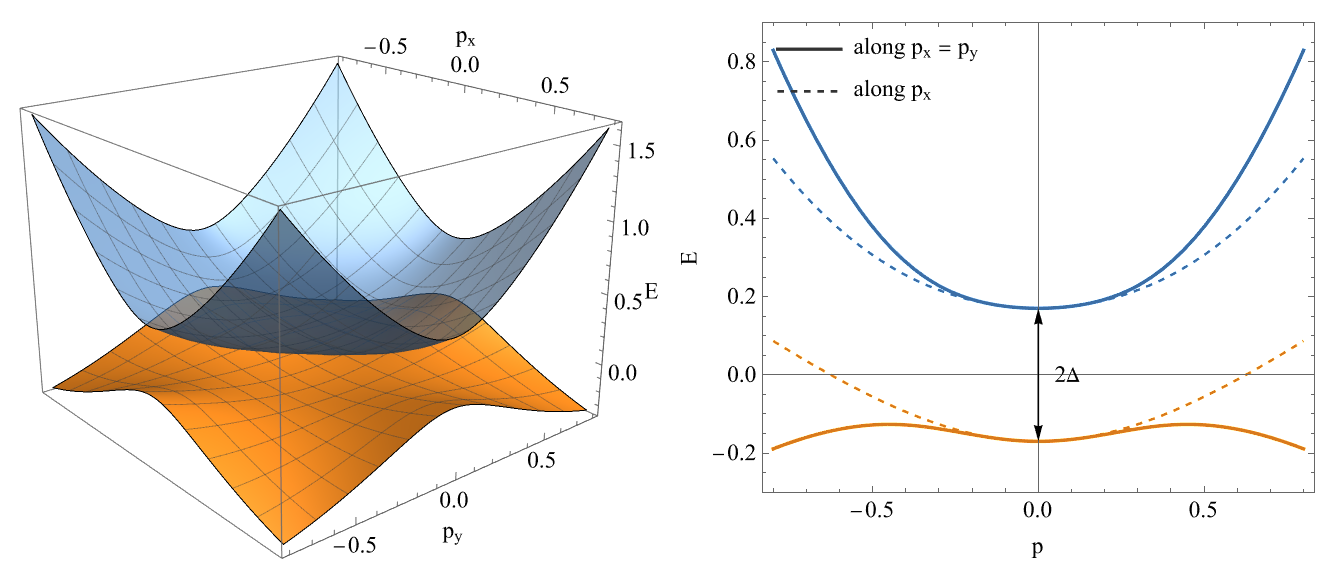
\includegraphics[width=\textwidth]{Gapped_Singular_Saddle.png}\caption{}\end{subfigure}\hfill
\begin{subfigure}{0.55\textwidth}\centering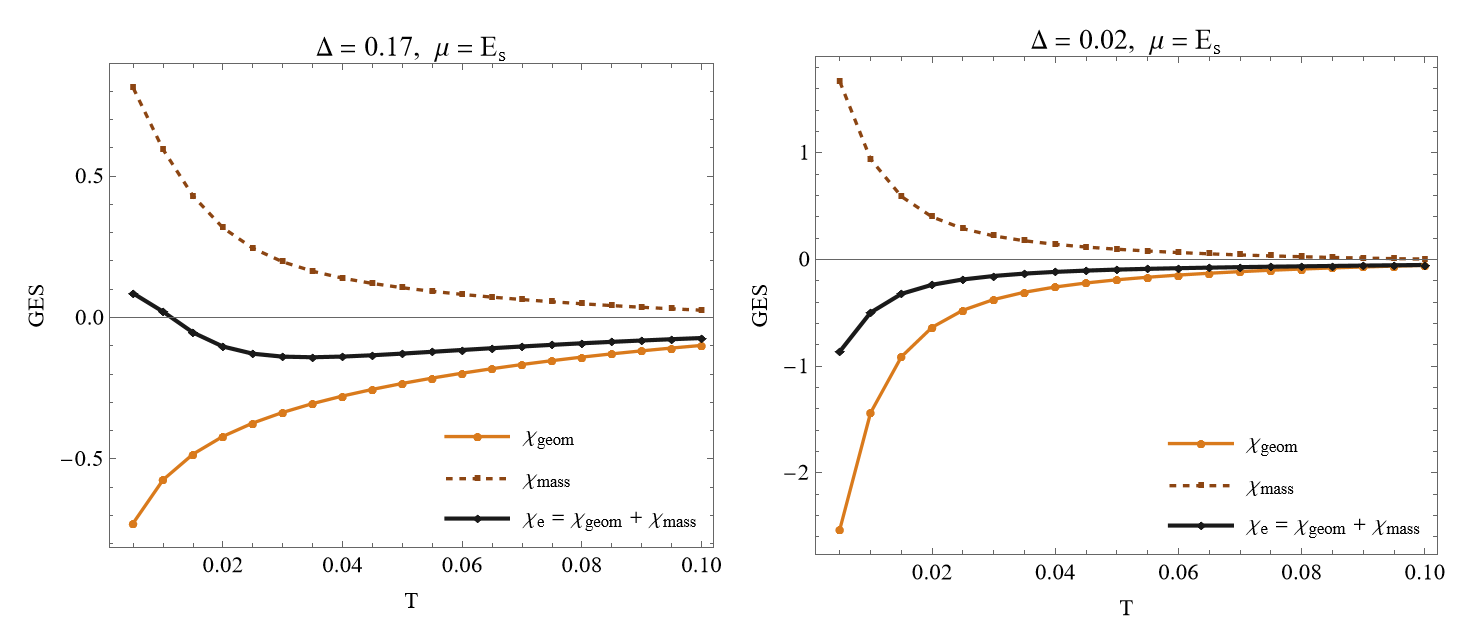
\includegraphics[width=\textwidth]{GES_Singular.png}\caption{}\end{subfigure}
\caption{Gapped singular saddle point. (a) Bands for $\Delta=0.17$ (gap $2\Delta$, model units). (b) GES against temperature at the saddle energy for $\Delta=0.17$ and $\Delta=0.02$: $\chig$, $\chim$ and $\chie=\chig+\chim$.}
% Check: assign red/blue to chi_geom / chi_mass to match your own notebook before submission.
\label{fig:bench}
\end{figure}

\end{document}
\end{document}